%Version 3.1 December 2024 -- Springer Nature LaTeX template (sn-article.tex)
%% Computer Networks Research Project, Phase 4. Two-column layout (template option iicol).

\documentclass[pdflatex,sn-mathphys-num,iicol]{sn-jnl}% Math and Physical Sciences Numbered Reference Style

%%%% Standard packages from the Springer Nature template
\usepackage{graphicx}%
\usepackage{multirow}%
\usepackage{amsmath,amssymb,amsfonts}%
\usepackage{amsthm}%
\usepackage{mathrsfs}%
\usepackage[title]{appendix}%
\usepackage{xcolor}%
\usepackage{textcomp}%
\usepackage{manyfoot}%
\usepackage{booktabs}%
\usepackage{algorithm}%
\usepackage{algorithmicx}%
\usepackage{algpseudocode}%
\usepackage{listings}%
%%%% Additional packages used in this manuscript
\usepackage{array}%
\usepackage{tikz}%
\usetikzlibrary{positioning,arrows.meta,fit,backgrounds,calc}%

\newcommand{\ms}{\,ms}
\newcolumntype{L}[1]{>{\raggedright\arraybackslash}p{#1}}

\raggedbottom

\begin{document}

\title[Lightweight Open-Set Detection for Encrypted-Port Flows]{Lightweight Open-Set Intrusion Detection for Encrypted-Port Network Flows: Unseen Attacks, CPU Cost, Cross-Dataset Transfer and Explainability}

\author*[1]{\fnm{Romaisa}}\email{i240061@isb.nu.edu.pk}
\equalcont{These authors contributed equally to this work.}

\author*[1]{\fnm{Maham} \sur{Anjum}}\email{i240053@isb.nu.edu.pk}
\equalcont{These authors contributed equally to this work.}

\affil*[1]{\orgdiv{Department of Artificial Intelligence and Data Science}, \orgname{National University of Computer and Emerging Sciences (FAST-NUCES)}, \orgaddress{\city{Islamabad}, \country{Pakistan}}}

\abstract{Encryption hides packet payloads, so intrusion detection must rely on flow metadata such as packet sizes, timing and TCP flags. Recent encrypted-traffic detectors report accuracies above 94\%, but most are evaluated with random splits, on GPUs and on a single dataset, and none combines unseen-attack detection, low CPU cost, cross-dataset transfer and explanations. This paper proposes a lightweight open-set detector, a 7,092-parameter multi-layer perceptron with a prototype-based open-set head, and compares it with seven re-implemented baselines on 241,109 cleaned encrypted-port flows from CIC-IDS-2017 and CSE-CIC-IDS2018, using temporal splits, validation-only thresholds at 1\% false-positive rate (FPR) and five seeds. On known attacks the detector reaches an AUROC of 0.922 (XGBoost: 0.950), but its realised test FPR is 5.5\% against 15.5\% for XGBoost, giving 34\% higher precision (0.710 vs.\ 0.529) and a higher F1 (0.679 vs.\ 0.651). It scores a flow in 0.38\ms{} on one CPU thread, 21$\times$ faster than Random Forest and 3.1$\times$ faster than XGBoost. Recalibration on 1,000 unlabeled benign flows restores the 1\% operating point on a new network (1.11\% and 1.02\% FPR), and Integrated Gradients explanations are faithful at a cost similar to detection. However, no method detects held-out attack families at 1\% FPR, and a random split alone raises Random Forest accuracy from 85.2\% to 95.9\%, showing that much reported accuracy comes from the evaluation protocol.}

\keywords{Encrypted traffic, Intrusion detection, Open-set recognition, Cross-dataset transfer, Explainable AI}

\maketitle

%%==================================%%
\section{Introduction}\label{sec:intro}
%%==================================%%

Most network traffic is now protected by TLS, SSH or QUIC, which removes the payload that signature-based intrusion detection systems (IDS) inspect. An IDS for encrypted traffic must therefore use metadata that stays visible: packet lengths, inter-arrival times, TCP flags, window sizes and volume. Recent work applies machine learning to this metadata through feature selection \cite{lee2026afs,xu2025pathsig}, graph neural networks \cite{liu2026fireg,li2026mtdecipher,yuan2025dcgl,liu2025gcnmha,okonkwo2025graph}, anomaly detection \cite{sattar2025etssl,haynes2025evade} and open-set or incremental learning \cite{yang2026ohce,cevallos2025hero,carillo2025fcil}.

These studies report 94--99\% accuracy, but the review conducted in Phases~1--2 of this project found that their evaluation rarely matches deployment. Most split flows at random, zero-day attacks are injected into training data \cite{sattar2025etssl}, thresholds are tuned on test scores \cite{haynes2025evade}, cost is reported per epoch \cite{yuan2025dcgl} or on a GPU \cite{yang2026ohce}, and explanations address closed-set classification \cite{xu2025pathsig,carillo2025fcil}. Such pitfalls are known in security machine learning \cite{arp2022dos}, and CIC-IDS-2017 has documented labelling problems \cite{engelen2021troubleshooting}.

The research gap is therefore: \emph{no reviewed method gives good accuracy, detection of unseen attack families and low CPU cost together, tested on encrypted traffic across datasets and with explanations for its alerts.} Four sub-gaps are tested: G1 (unseen families), G2 (CPU cost), G3 (cross-dataset transfer) and G5 (explanations). Drift with new classes (G4, Phase~2) was removed from scope. The contributions are:
\begin{itemize}
\item a lightweight open-set detector (7,092 parameters, 0.38\ms{} per flow on one CPU thread);
\item a leakage-controlled benchmark from two public datasets with temporal splits, a duplicate and label-conflict audit and validation-only thresholds, on which seven baselines are re-implemented under identical conditions;
\item four protocols (closed-set, leave-one-family-out, cross-dataset, CPU cost) with five seeds, confidence intervals, significance tests and pre-registered criteria;
\item a label-free recalibration that restores the 1\% FPR on a new network, and faithful, low-cost explanations of alerts;
\item two findings for the field: a random split alone adds 10.7 points of accuracy, and no method detects unseen families from flow statistics at 1\% FPR.
\end{itemize}
Section~\ref{sec:related} reviews related work, Sections~\ref{sec:method}--\ref{sec:setup} present the method and setup, Sections~\ref{sec:results}--\ref{sec:ablation} report results, comparisons and ablations, and Sections~\ref{sec:discussion}--\ref{sec:conclusion} discuss and conclude.

%%==================================%%
\section{Related Work}\label{sec:related}
%%==================================%%

Table~\ref{tab:related} summarises the reviewed studies by approach.

\textbf{Feature-based detectors:} Gradient-relevance feature selection \cite{lee2026afs} and path-signature features \cite{xu2025pathsig} show that compact features work well, but only for closed-set classification on single datasets.

\textbf{Graph-based detectors:} FIRE-G \cite{liu2026fireg}, MTDecipher \cite{li2026mtdecipher}, DC-GL \cite{yuan2025dcgl}, GCN-MHA \cite{liu2025gcnmha} and the framework of Okonkwo et al.\ \cite{okonkwo2025graph} model relations between flows or hosts and reach 96--99\% accuracy, but they are costly (e.g.\ 450k parameters and 15.2\ms{} per sample for GCN-MHA) and use random closed-set splits.

\textbf{Anomaly-based detectors:} ET-SSL \cite{sattar2025etssl} scores distance to a contrastive centroid and EVADE \cite{haynes2025evade} fits an Elliptic Envelope on benign traffic (1.8\ms{} per flow). They need no attack labels, but their zero-days are injected into training or their thresholds set on test data.

\textbf{Open-set and incremental learning:} OHCE \cite{yang2026ohce} rejects unknown traffic with class hash centres (GPU cost only, rebuilt benchmark); HERO \cite{cevallos2025hero} detects held-out classes on non-encrypted IoT data; federated incremental learning \cite{carillo2025fcil} and E-MGFlow \cite{wu2025emgflow} address application classes and private data.

\textbf{Position of this work:} The proposed method borrows prototypes from OHCE and HERO and a benign boundary from EVADE and ET-SSL, but it is evaluated on held-out families, temporal splits and a second dataset, on the same data and hardware as all baselines, with end-to-end CPU cost and explanations of the detector's own alerts.

\begin{table*}[t]
\caption{Summary of the reviewed studies (results as reported by the authors; RS: random split).}\label{tab:related}
\footnotesize
\setlength{\tabcolsep}{3pt}
\begin{tabular}{@{}L{1.8cm}L{3.2cm}L{3.5cm}L{3.0cm}L{3.2cm}@{}}
\toprule
Study & Dataset(s) & Method & Reported result & Main limitation \\
\midrule
AFS \cite{lee2026afs} & CIRA-CIC-DoHBrw2020 & Gradient-relevance feature selection & 88.0\% detection rate & One dataset, synthetic noise \\
Path-sig.\ \cite{xu2025pathsig} & CTU-HTTPS, ISCX, QUIC2019 & Path signatures + RF/LightGBM & 91\% fewer features & Closed-set only \\
FIRE-G \cite{liu2026fireg} & ToN-IoT, CICIoT2023, USTC & GAT/RGAT flow-interaction graphs & F1 99.41\% (USTC) & High cost, no latency \\
MTDecipher \cite{li2026mtdecipher} & USTC-TFC, MCFP & Bi-GRU + GraphSAGE, multi-task & Best of 8 baselines & Synthetic obfuscation \\
DC-GL \cite{yuan2025dcgl} & CIC-IDS-2017, CIC-AndMal2017 & Separable GCN + LSTM & Acc.\ 97.29\% (RS) & RS, cost per epoch \\
GCN-MHA \cite{liu2025gcnmha} & ISCX-VPN2016, USTC, Darknet & GCN + 8-head attention & Acc.\ 98.79\%, 15.2\ms & VPN apps as malicious \\
Graph fw.\ \cite{okonkwo2025graph} & ISCX-VPN/Tor, USTC & GNN + GNNExplainer & Acc.\ 96.0--99.4\% & Per-dataset, closed-set \\
ET-SSL \cite{sattar2025etssl} & CIC-Darknet2020, ISCX, UNSW-NB15 & Contrastive encoder + centroid & Acc.\ 94.3--96.8\% & Injected zero-days \\
EVADE \cite{haynes2025evade} & CIC-IoT-2023 & PCA + Elliptic Envelope & F1 0.982, 1.8\ms & Threshold set on test \\
OHCE \cite{yang2026ohce} & USTC-TFC2016, CIC-IDS-2018-R & CvT + multi-prototype hash centres & Open-set acc.\ 94.4--97.0\% & Rebuilt data, GPU cost \\
HERO \cite{cevallos2025hero} & BoT-IoT, Edge-IIoTset & GATv2 + CNN + prototypes & Zero-day bal.\ acc.\ 0.93--0.99 & Not encrypted, GPU \\
FCIL \cite{carillo2025fcil} & CESNET-TLS22, MIRAGE19 & Federated CIL + SHAP & Macro-F1 $\approx$79--82\% & App.\ classes only \\
E-MGFlow \cite{wu2025emgflow} & DataCon2020/21, private & MHA + BiLSTM fusion & F1 93.55\%, FPR 6.5\% & Private data, 140\ms \\
\midrule
This work & CIC-IDS-2017, CSE-CIC-IDS2018 & MLP + prototype open-set head & AUROC 0.922, 0.38\ms{} (CPU) & Unseen families missed \\
\botrule
\end{tabular}
\end{table*}

%%==================================%%
\section{Proposed Methodology}\label{sec:method}
%%==================================%%

\textbf{Problem formulation:} Let $\mathbf{x}\in\mathbb{R}^{d}$ be the CICFlowMeter statistics \cite{lashkari2017cicflowmeter} of a flow on an encrypted port and $y\in\{0,\dots,K-1\}$ its family, with $0$ benign and $\mathcal{A}=\{1,\dots,K-1\}$ the known attacks. A test flow may belong to an unseen family $u\notin\mathcal{A}$. The detector outputs a score $s(\mathbf{x})$ and an alert $\mathbf{1}[s(\mathbf{x})>\tau]$, where $\tau$ is set on benign validation flows $\mathcal{V}_{b}$ for a target FPR $\alpha=1\%$:
\begin{equation}
\tau = Q_{1-\alpha}\big(\{s(\mathbf{x}_i):\mathbf{x}_i\in\mathcal{V}_{b}\}\big),\label{eq:tau}
\end{equation}
with $Q_p$ the empirical $p$-quantile. Figure~\ref{fig:arch} shows the pipeline.

\begin{figure*}[t]
\centering
\resizebox{0.84\textwidth}{!}{%
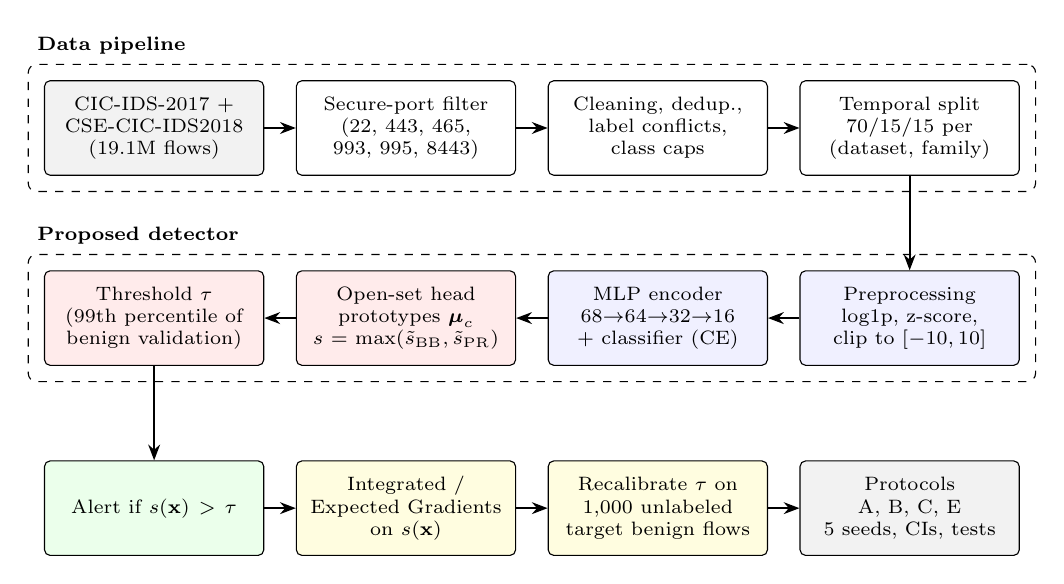
\begin{tikzpicture}[
  node distance=12mm and 4mm,
  box/.style={draw, rounded corners=2pt, align=center, font=\scriptsize, minimum height=12mm, text width=2.55cm, fill=white},
  arr/.style={-{Stealth[length=2mm]}, thick},
  grp/.style={draw, dashed, rounded corners=3pt, inner sep=2mm}]
\node[box, fill=gray!10] (data) {CIC-IDS-2017 +\\CSE-CIC-IDS2018\\(19.1M flows)};
\node[box, right=of data] (filter) {Secure-port filter\\(22, 443, 465,\\993, 995, 8443)};
\node[box, right=of filter] (clean) {Cleaning, dedup.,\\label conflicts,\\class caps};
\node[box, right=of clean] (split) {Temporal split\\70/15/15 per\\(dataset, family)};
\node[box, below=of split, fill=blue!6] (pre) {Preprocessing\\log1p, z-score,\\clip to $[-10,10]$};
\node[box, left=of pre, fill=blue!6] (enc) {MLP encoder\\$68{\to}64{\to}32{\to}16$\\+ classifier (CE)};
\node[box, left=of enc, fill=red!8] (head) {Open-set head\\prototypes $\boldsymbol{\mu}_c$\\$s=\max(\tilde{s}_{\mathrm{BB}},\tilde{s}_{\mathrm{PR}})$};
\node[box, left=of head, fill=red!8] (thr) {Threshold $\tau$\\(99th percentile of\\benign validation)};
\node[box, below=of thr, fill=green!8] (alert) {Alert if $s(\mathbf{x})>\tau$};
\node[box, right=of alert, fill=yellow!12] (xai) {Integrated /\\Expected Gradients\\on $s(\mathbf{x})$};
\node[box, right=of xai, fill=yellow!12] (recal) {Recalibrate $\tau$ on\\1,000 unlabeled\\target benign flows};
\node[box, right=of recal, fill=gray!10] (eval) {Protocols A, B, C, E\\5 seeds, CIs, tests};
\draw[arr] (data) -- (filter); \draw[arr] (filter) -- (clean); \draw[arr] (clean) -- (split);
\draw[arr] (split) -- (pre); \draw[arr] (pre) -- (enc); \draw[arr] (enc) -- (head); \draw[arr] (head) -- (thr);
\draw[arr] (thr) -- (alert); \draw[arr] (alert) -- (xai); \draw[arr] (xai) -- (recal); \draw[arr] (recal) -- (eval);
\begin{scope}[on background layer]
\node[grp, fit=(data)(split)] (g1) {};
\node[grp, fit=(pre)(thr)] (g2) {};
\end{scope}
\node[font=\scriptsize\bfseries, anchor=south west] at (g1.north west) {Data pipeline};
\node[font=\scriptsize\bfseries, anchor=south west] at (g2.north west) {Proposed detector};
\end{tikzpicture}}
\caption{Architecture of the proposed approach: leakage-controlled data pipeline, detector (blue: representation; red: open-set scoring), and explanation and label-free recalibration (yellow), which address G5 and G3.}\label{fig:arch}
\end{figure*}

\textbf{Preprocessing:} After removing constant columns ($d=68$), heavy-tailed features are transformed by $\phi_j(x)=\operatorname{sign}(x)\log(1+|x|)$, then standardised with training statistics and clipped:
\begin{equation}
\tilde{x}_j=\operatorname{clip}\big((\phi_j(x_j)-m_j)/\sigma_j,\,-10,\,10\big).\label{eq:pre}
\end{equation}
The port is not used as a feature except in one ablation.

\textbf{Encoder and classifier:} The encoder $f_\theta:\mathbb{R}^{68}\to\mathbb{R}^{16}$ has ReLU layers of 64 and 32 units and a linear 16-unit output $\mathbf{z}$. A linear classifier gives $p(y\,|\,\mathbf{x})=\operatorname{softmax}(g_\psi(\mathbf{z}))$. The model (7,092 parameters) is trained with class-weighted cross-entropy
\begin{equation}
\mathcal{L}=-\frac{1}{N}\sum_{i=1}^{N} w_{y_i}\log p(y_i\,|\,\mathbf{x}_i),\quad w_c=\sqrt{\frac{N}{K\,n_c}},\label{eq:loss}
\end{equation}
where $n_c$ is the size of class $c$; the square root up-weights rare classes without letting them dominate.

\textbf{Open-set head:} Class prototypes $\boldsymbol{\mu}_c$ are the mean training embeddings \cite{snell2017proto}. With $d_b=\lVert\mathbf{z}-\boldsymbol{\mu}_0\rVert_2$ (benign) and $d_a=\min_{c\in\mathcal{A}}\lVert\mathbf{z}-\boldsymbol{\mu}_c\rVert_2$ (nearest attack), two scores are computed:
\begin{equation}
s_{\mathrm{BB}}=d_b,\qquad s_{\mathrm{PR}}=\log(d_b+\epsilon)-\log(d_a+\epsilon).\label{eq:raw}
\end{equation}
The \emph{Benign-boundary} score flags flows far from normal traffic (which could include unseen families); the \emph{Proto-ratio} score flags flows closer to an attack than to benign. Each is calibrated on benign validation embeddings, $\tilde{s}_k=(s_k-\mathrm{med}_k)/(1.4826\,\mathrm{MAD}_k)$, and combined:
\begin{equation}
s(\mathbf{x})=\max\big(\tilde{s}_{\mathrm{BB}},\,\tilde{s}_{\mathrm{PR}}\big).\label{eq:score}
\end{equation}

\begin{algorithm}[t]
\caption{Training, scoring and recalibration}\label{alg:detector}
\footnotesize
\begin{algorithmic}[1]
\Require training set $\mathcal{T}$, validation set $\mathcal{V}$, FPR $\alpha$
\State Fit Eq.~(\ref{eq:pre}) on $\mathcal{T}$; compute $w_c$ (Eq.~\ref{eq:loss})
\State Train $f_\theta,g_\psi$ with Adam (batch 512, $\le$30 epochs, early stop 5)
\State $\boldsymbol{\mu}_c\gets$ mean of $f_\theta(\mathbf{x})$ over class $c$ in $\mathcal{T}$
\State $\mathrm{med}_k,\mathrm{MAD}_k\gets$ statistics of $s_k$ on benign $\mathcal{V}$
\State $\tau\gets Q_{1-\alpha}$ of $s(\mathbf{x})$ on benign $\mathcal{V}$ \Comment{Eq.~(\ref{eq:tau})}
\Function{Score}{$\mathbf{x}$} \Return $s(\mathbf{x})$ (Eq.~\ref{eq:score}), alert $\mathbf{1}[s>\tau]$ \EndFunction
\Function{Recalibrate}{unlabeled benign target flows $\mathcal{U}$}
  \State $\tau\gets Q_{1-\alpha}(\{s(\mathbf{x}):\mathbf{x}\in\mathcal{U}\})$ \Comment{G3}
\EndFunction
\end{algorithmic}
\end{algorithm}

\textbf{Explanations and recalibration:} Explanations are computed on $s(\mathbf{x})$ itself. Integrated Gradients (IG) \cite{sundararajan2017ig} attributes the score difference to a benign baseline $\tilde{\mathbf{x}}'$,
\begin{equation}
\mathrm{IG}_j=(\tilde{x}_j-\tilde{x}'_j)\int_{0}^{1}\frac{\partial s(\tilde{\mathbf{x}}'+t(\tilde{\mathbf{x}}-\tilde{\mathbf{x}}'))}{\partial \tilde{x}_j}\,dt,\label{eq:ig}
\end{equation}
with $\sum_j\mathrm{IG}_j=s(\tilde{\mathbf{x}})-s(\tilde{\mathbf{x}}')$; Expected Gradients (EG) \cite{erion2021eg} averages over 64 benign references. Attributions are also grouped into 42 correlation clusters of near-duplicate features. On a new network, \textsc{Recalibrate} (Algorithm~\ref{alg:detector}) resets $\tau$ from unlabeled traffic assumed benign. A later version (v3) adds per-network quantile preprocessing, daily recalibration and a \emph{Hybrid} detector (maximum of the benign percentiles of $s$ and of a Random Forest).

\textbf{Changes after Phase~2:} The public CSVs contain flow statistics but no packets or TLS fields, so the planned 10-packet CNN/GRU became an MLP on flow statistics and TLS filtering became a secure-port filter; random 5-fold cross-validation became a temporal split to avoid leakage; drift windows (G4) were dropped; feature selection uses Random Forest ranking; hash-centre and graph baselines are compared through reported results; and cost is measured on a laptop CPU instead of an edge device. Success criteria for each version were fixed before it was run, and all versions are reported.

%%==================================%%
\section{Experimental Setup}\label{sec:setup}
%%==================================%%

\textbf{Datasets:} The study uses the Kaggle releases \cite{kaggle2017,kaggle2018} of CIC-IDS-2017 \cite{sharafaldin2018cicids} (2,830,743 flows) and CSE-CIC-IDS2018 (16,233,002 flows), mapped to 76 common CICFlowMeter features (23 volume, 22 timing, 19 length, 12 flag). As neither marks encrypted flows, only flows on ports $\{22, 443, 465, 993, 995, 8443\}$ are kept (2,752,911 flows, 14\%). The remaining families are benign, SSH brute force (both datasets), PortScan (2017) and Infiltration (2018); DoS/DDoS run on port 80 and drop out. Other Phase~2 datasets were unsuitable: no flow in the nine readable USTC-TFC2016 captures contained a TLS handshake record (checked with Scapy, even in Gmail, whose traffic largely goes to port 443), and every CIC-Darknet2020 flow is labelled Non-Tor with only application categories. In CIC-IDS-2017, ports 443/8443 alone contain a single attack type (325 PortScan flows), which motivated the six-port filter and the second dataset.

\textbf{Cleaning and splits:} The cleaning step removed 1,961 rows with infinite or missing values, 40 negative durations, 470,510 duplicates and 23,262 label conflicts (flows whose features appear with two labels); 39\% of 2018 infiltration flows were identical to benign flows, consistent with known labelling issues \cite{engelen2021troubleshooting}. Benign and SSH flows were capped per dataset (about 100,000 and 20,000), sampled evenly across files. Each (dataset, family) group was split by time into 70/15/15\% train/validation/test (2017 by file and row order, as it lacks timestamps). All scalers, selections, prototypes and thresholds were fitted on training or validation data, and no identical feature vectors remained across labels, splits or datasets. Table~\ref{tab:data} gives the final 241,109 flows (83\% benign).

\begin{table}[t]
\caption{Final dataset (temporal split).}\label{tab:data}
\footnotesize
\setlength{\tabcolsep}{3pt}
\begin{tabular}{@{}llrrr@{}}
\toprule
Dataset & Family & Train & Val. & Test \\
\midrule
2017 & Benign & 70,000 & 15,000 & 15,000 \\
2017 & PortScan & 327 & 70 & 69 \\
2017 & SSH brute force & 2,254 & 483 & 482 \\
2018 & Benign & 69,999 & 15,000 & 14,999 \\
2018 & Infiltration & 12,199 & 2,614 & 2,613 \\
2018 & SSH brute force & 14,000 & 3,000 & 3,000 \\
\midrule
\multicolumn{2}{@{}l}{Total (241,109)} & 168,779 & 36,167 & 36,163 \\
\botrule
\end{tabular}
\end{table}

\textbf{Protocols:} \emph{A (closed-set):} all families seen in training. \emph{B (leave-one-family-out, G1):} one attack family is removed from training and validation and tested as unseen. \emph{C (cross-dataset, G3):} train on one dataset, test on the other with the source threshold and after recalibration, against criteria fixed in advance: (C1) FPR $\le$2\% both ways; (C2) SSH AUROC drop $\le$0.05; (C3) recalibration reduces FPR error; (C4) FPR $<\max(2\%,2\times$ in-source) under a time-ordered design. \emph{E (cost, G2):} single-thread end-to-end latency over 1,000 flows, throughput in batches of 4,096, model size and training time.

\textbf{Baselines:} All baselines share features, splits, hardware and Eq.~(\ref{eq:tau}): Random Forest (100 trees, depth 20) \cite{pedregosa2011sklearn} and XGBoost (100 trees) \cite{chen2016xgboost} with the same class weights; Isolation Forest \cite{liu2008iforest} and an EVADE-style PCA + Elliptic Envelope \cite{rousseeuw1999mcd,haynes2025evade} on benign flows; and three scores of the same MLP: maximum softmax probability (MSP) \cite{hendrycks2017msp}, benign Mahalanobis distance \cite{lee2018mahalanobis} and MLP-closed ($1-p(\text{benign})$).

\textbf{Metrics and implementation:} Since an always-benign detector already scores 83\% accuracy, the evaluation reports AUROC, PR-AUC, TPR at 1\% FPR, realised test FPR, precision and F1, plus accuracy and macro-F1 for classification. Results are means over seeds 0--4 (0--2 for ablations) with bootstrap 95\% intervals (200 resamples) and Wilcoxon signed-rank tests. The MLP uses Adam (learning rate $10^{-3}$, weight decay $10^{-5}$). Experiments ran on a Windows laptop with an Intel Core i5-8365U CPU (1.60\,GHz, 4 cores, 8 threads) and 8\,GB RAM, using Python 3.13.9, NumPy 2.4.6, pandas 3.0.6, scikit-learn, XGBoost, PyTorch \cite{paszke2019pytorch} and SHAP \cite{lundberg2017shap}; Protocols A and B with all methods and seeds take about 20 minutes.

%%==================================%%
\section{Results and Analysis}\label{sec:results}
%%==================================%%

\textbf{Known attacks (Protocol A):} Table~\ref{tab:protA} shows that XGBoost ranks attacks best (AUROC 0.950, 95\% CI $[0.948,0.952]$) and the proposed detector reaches 0.922 ($[0.919,0.926]$). The 1\% validation threshold, however, does not hold on later test days: realised FPR is 15.5\% for XGBoost and 16.8\% for Random Forest but 5.5\% for the proposed detector, which therefore has higher precision and F1 than the tree ensembles, MLP-closed and the Hybrid. Mahalanobis and the Benign-boundary component alone are more conservative (FPR 2.4\% and 1.4\%) but rank attacks worse (AUROC 0.771 and 0.823). Benign-only detectors and MSP are near chance. In classification, the tree models reach 85.2--85.4\% accuracy (macro-F1 0.821) and the MLP 82.3\% (0.788). SSH and PortScan are easy (AUROC $\approx$1.0), but 37--42\% of infiltration flows are predicted benign by every model (best infiltration AUROC 0.775).

\begin{table}[t]
\caption{Protocol A: known-attack detection at the 1\% validation threshold (mean, with AUROC $\pm$ std, over 5 seeds).}\label{tab:protA}
\footnotesize
\setlength{\tabcolsep}{2pt}
\begin{tabular}{@{}lccccc@{}}
\toprule
Method & AUROC & TPR@1\% & FPR & Prec. & F1 \\
\midrule
XGBoost & \textbf{0.950}$\pm$.000 & \textbf{0.605} & 15.5\% & 0.529 & 0.651 \\
Random Forest & 0.940$\pm$.002 & 0.227 & 16.8\% & 0.515 & 0.646 \\
Hybrid (v3) & 0.938$\pm$.001 & 0.482 & 15.9\% & 0.521 & 0.644 \\
MLP-closed & 0.932$\pm$.002 & 0.571 & 8.4\% & 0.625 & 0.649 \\
\textbf{Proposed} & 0.922$\pm$.003 & 0.556 & 5.5\% & 0.710 & 0.679 \\
Mahalanobis & 0.771$\pm$.012 & 0.520 & 2.4\% & \textbf{0.835} & \textbf{0.682} \\
Isolation Forest & 0.532$\pm$.031 & 0.014 & 2.1\% & 0.163 & 0.035 \\
MSP & 0.521$\pm$.033 & 0.010 & 2.3\% & 0.185 & 0.045 \\
Elliptic Env. & 0.433$\pm$.002 & 0.000 & \textbf{0.9\%} & 0.000 & 0.000 \\
\botrule
\end{tabular}
\end{table}

\textbf{Unseen families (Protocol B, G1):} No method detects a held-out family at 1\% FPR (Table~\ref{tab:protB}, Figure~\ref{fig:auroc}). The proposed detector flags 0.9\% of unseen infiltration and none of unseen PortScan or SSH, and its unseen-SSH AUROC (0.278) is below chance, i.e.\ brute-force sessions look \emph{more} normal than benign flows. Isolation Forest ranks unseen PortScan well (0.944) but flags only 12.5\% of it. Closed-set macro-F1 remains 0.73--0.96, so the open-set head does not harm known classes. Over 15 paired (family, seed) runs the proposed detector is below every baseline, but significantly only against Isolation Forest (Wilcoxon $p=0.003$; $p\ge0.055$ otherwise). G1 is not achieved.

\begin{table}[t]
\caption{Protocol B: AUROC on each held-out family (share flagged at the 1\% threshold).}\label{tab:protB}
\footnotesize
\setlength{\tabcolsep}{2.5pt}
\begin{tabular}{@{}lccc@{}}
\toprule
Method & Infiltration & PortScan & SSH \\
\midrule
Proposed & 0.502 (0.9\%) & 0.470 (0.0\%) & 0.278 (0.0\%) \\
Random Forest & 0.475 (1.5\%) & 0.773 (3.6\%) & 0.324 (0.0\%) \\
XGBoost & 0.307 (2.1\%) & 0.654 (16.2\%) & 0.404 (0.1\%) \\
Isolation Forest & 0.480 (1.7\%) & \textbf{0.944} (12.5\%) & 0.526 (0.0\%) \\
MSP & 0.359 (1.2\%) & 0.602 (0.3\%) & \textbf{0.643} (0.0\%) \\
\botrule
\end{tabular}
\end{table}

\begin{figure}[t]
\centering
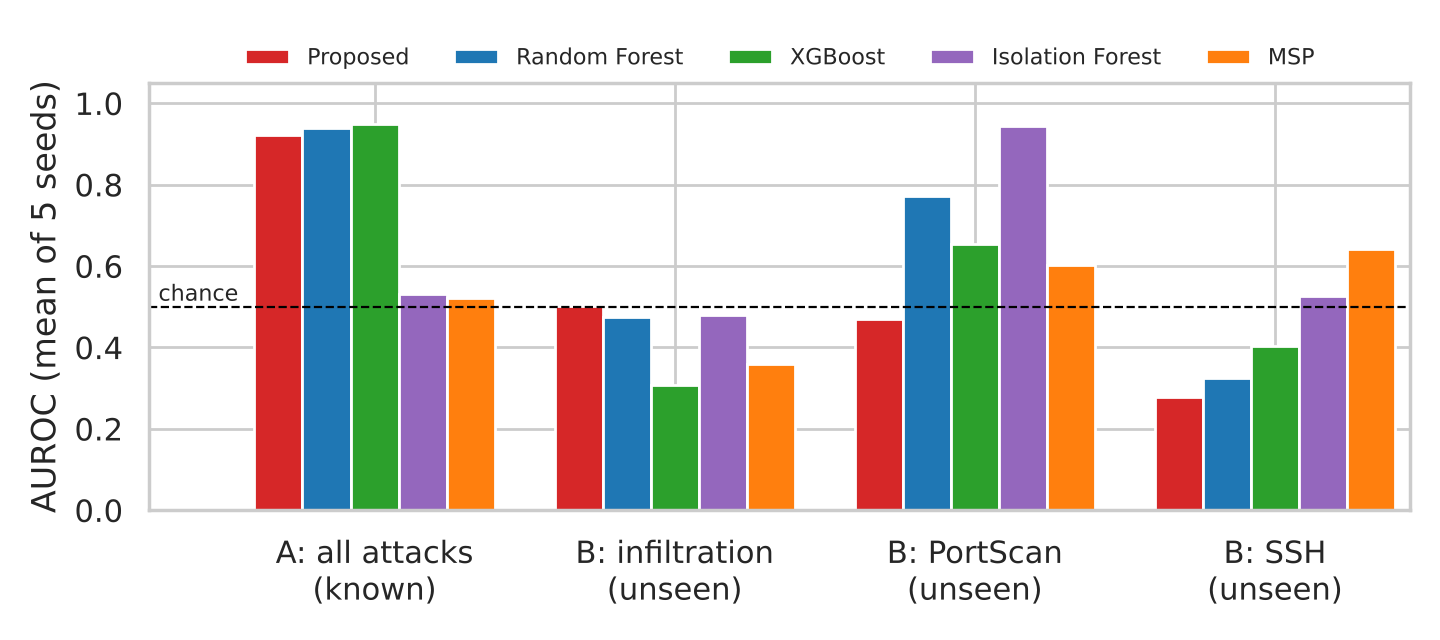
\includegraphics[width=\columnwidth]{figs/fig_auroc_known_unseen.png}
\caption{AUROC on known attacks (Protocol A) and on each held-out family (Protocol B).}\label{fig:auroc}
\end{figure}

\textbf{Cross-dataset transfer (Protocol C, G3):} With the source threshold, the proposed detector keeps 0.9\% FPR from 2017 to 2018 but reaches 3.2\% in reverse (tree models: 3.1--6.6\%), and SSH AUROC falls from 0.999 in-source to 0.69 and 0.81. Even within a dataset, a 1\% validation threshold gives about 6\% on test days. Table~\ref{tab:protC} reports the three versions. In v2, 1,000 unlabeled benign flows restore the operating point (1.11\% and 1.02\%; Figure~\ref{fig:recal}), even with 5\% attack contamination (1.09--1.13\%). The cross-dataset part of the remaining error is only 0.11 and 0.02 points, against 0.48 and 3.73 points of within-network time drift, so drift dominates; daily recalibration (v3) keeps the Hybrid at 1.0--1.5\% FPR. SSH transfer (C2) fails in every version except 2017$\to$2018 for the Hybrid. G3 is partly achieved (3/4 criteria).

\begin{table}[t]
\caption{Protocol C: transfer against pre-registered criteria.}\label{tab:protC}
\footnotesize
\setlength{\tabcolsep}{2.5pt}
\begin{tabular}{@{}lcccc@{}}
\toprule
 & \multicolumn{2}{c}{Benign FPR} & SSH AUROC & \\
Version (detector) & 17$\to$18 & 18$\to$17 & drop & Met \\
\midrule
v1 (Proposed) & 5.0\% & 1.1\% & 0.60 / 0.30 & 0/3 \\
v2 (Proposed) & 1.11\% & \textbf{1.02\%} & 0.77 (17$\to$18) & 3/4 \\
v3 (Hybrid) & \textbf{1.09\%} & 1.54\% & \textbf{0.014} (17$\to$18) & 3/4 \\
\botrule
\end{tabular}
\end{table}

\begin{figure}[t]
\centering
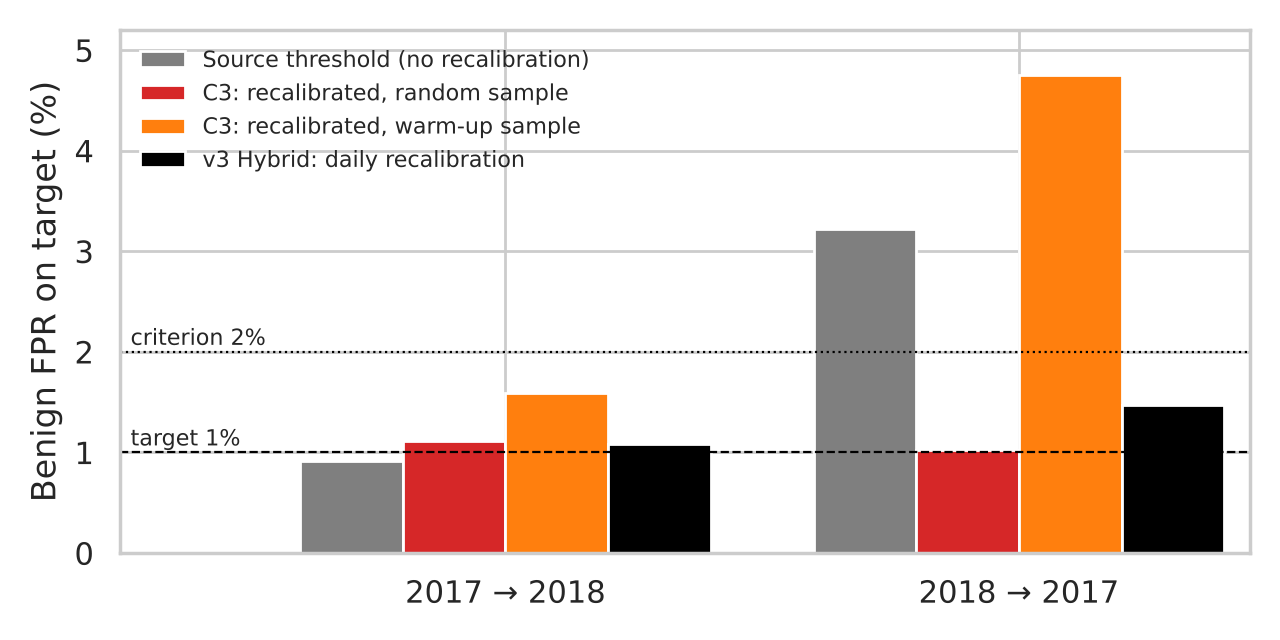
\includegraphics[width=\columnwidth]{figs/fig_recalibration.png}
\caption{Benign FPR on the other dataset with the source threshold, after recalibration on 1,000 unlabeled benign flows, and with daily recalibration (v3 Hybrid).}\label{fig:recal}
\end{figure}

\textbf{CPU cost (Protocol E, G2):} The proposed detector needs 0.38\ms{} per flow and 0.03\,MB (Table~\ref{tab:cost}), 21$\times$ faster than Random Forest and 3.1$\times$ faster than XGBoost; only MLP-closed, which shares its network, is faster. The v3 quantile preprocessing raises latency to 10.7\ms. Figure~\ref{fig:cost} shows that no method is both cheap and good on unseen families. G2 is achieved on a laptop CPU.

\begin{table}[t]
\caption{Protocol E: single-thread CPU cost per flow.}\label{tab:cost}
\footnotesize
\setlength{\tabcolsep}{2.5pt}
\begin{tabular}{@{}lrrrr@{}}
\toprule
Method & p50 (ms) & p95 (ms) & Flows/s & MB \\
\midrule
\textbf{Proposed} & 0.38 & 0.49 & 172,436 & \textbf{0.03} \\
MLP-closed & \textbf{0.24} & \textbf{0.33} & \textbf{189,674} & \textbf{0.03} \\
Elliptic Env. & 0.99 & 1.68 & 171,657 & 0.21 \\
XGBoost & 1.18 & 1.86 & 64,163 & 0.95 \\
Random Forest & 8.05 & 11.85 & 41,965 & 46.28 \\
Isolation Forest & 9.59 & 12.41 & 54,637 & 1.40 \\
Hybrid (v3) & 10.70 & 13.62 & 22,894 & 46.30 \\
\botrule
\end{tabular}
\end{table}

\begin{figure}[t]
\centering
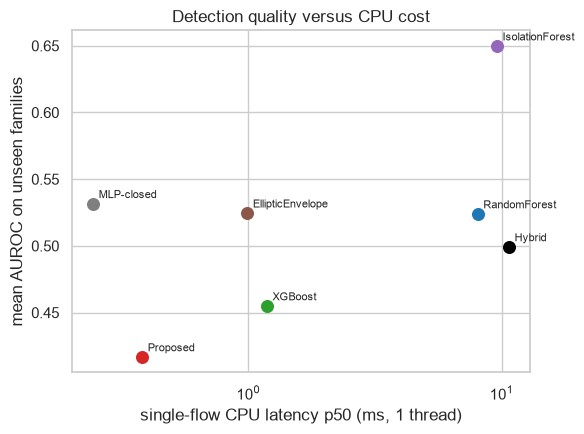
\includegraphics[width=0.85\columnwidth]{figs/fig_quality_vs_cost.png}
\caption{Mean unseen-family AUROC (Protocol B) against CPU latency.}\label{fig:cost}
\end{figure}

\textbf{Explainability (G5):} A TreeSHAP surrogate copies 99.8\% of the detector's decisions but disagrees with KernelSHAP on the real detector (top-10 Jaccard 0.11), so it was rejected. Gradient explanations on the detector itself are \emph{faithful}: replacing the top-10 IG features with benign values removes every unseen-family alert, against 35\% for random features (Figure~\ref{fig:xai}, left); \emph{complete} within about 2\%; \emph{stable} across seeds once grouped into clusters (Jaccard 0.79 and 0.73); and \emph{cheap} (p95 1.47\ms{}, similar to scoring, against 34.8\ms{} for KernelSHAP). As a qualitative example, alerts on unseen infiltration rest mainly on forward TCP header and window features (\texttt{fwd\_header\_len}, \texttt{min\_seg\_size\_fwd}, \texttt{init\_win\_fwd}; Figure~\ref{fig:xai}, right), which tells an analyst that these flows were flagged for their TCP header and window behaviour. The detector also relies on clusters that shift more between datasets (KS 0.22--0.27 vs.\ 0.19 on average), which explains its weak SSH transfer. Because G1 fails, few unseen alerts exist to explain (103 in v1). The best version passes 5 of 6 criteria; G5 is partly achieved.

\begin{figure*}[t]
\centering
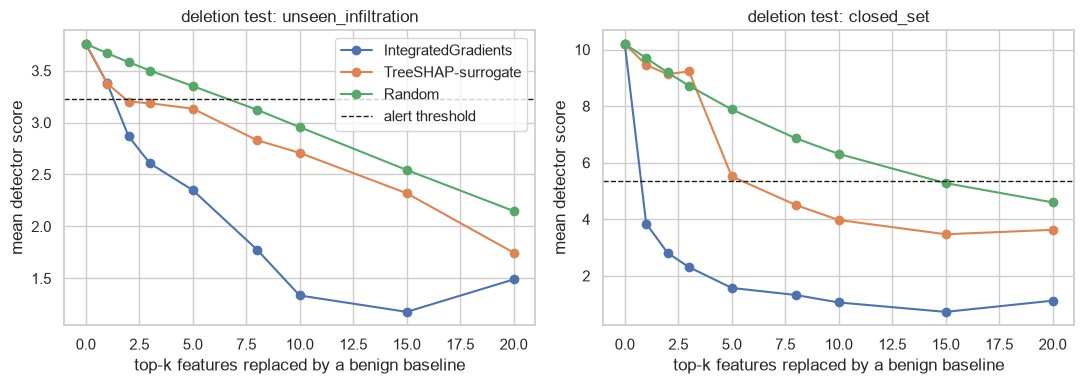
\includegraphics[height=4.0cm]{figs/fig_deletion.png}\hfill
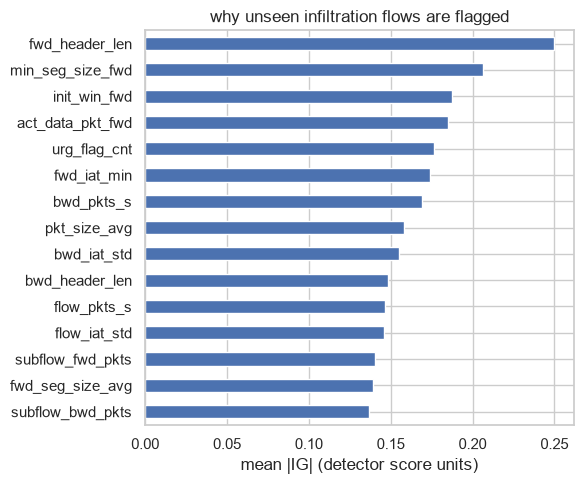
\includegraphics[height=4.0cm]{figs/fig_ig_features.png}
\caption{Left: deletion test; the detector score drops fastest when the top IG-ranked features are replaced by benign values. Right: qualitative example, mean $|\mathrm{IG}|$ of the features behind alerts on unseen infiltration flows.}\label{fig:xai}
\end{figure*}

\textbf{Error analysis:} False alarms concentrate on the 2018 infiltration days (FPR 17.9\% and 14.6\%, against 0.2--0.3\% on 2017 days). Recall is 100\% for PortScan, 86.7--99.8\% for SSH and 24\% for infiltration; missed infiltration flows have larger forward packets (+1.7 std) and irregular timing, resembling ordinary HTTPS sessions.

%%==================================%%
\section{Comparison with Base Papers}\label{sec:comparison}
%%==================================%%

The base papers are OHCE \cite{yang2026ohce}, DC-GL \cite{yuan2025dcgl}, ET-SSL \cite{sattar2025etssl}, EVADE \cite{haynes2025evade} and GCN-MHA \cite{liu2025gcnmha} (Table~\ref{tab:base}). Table~\ref{tab:quant} compares results; asterisked values are reported by the original authors on other data and hardware, while daggered rows were re-implemented on the data of this study.

\begin{table*}[t]
\caption{Summary of the base papers.}\label{tab:base}
\footnotesize
\setlength{\tabcolsep}{2pt}
\begin{tabular}{@{}L{1.9cm}L{2.0cm}L{2.5cm}L{2.2cm}L{1.8cm}L{2.5cm}L{2.1cm}@{}}
\toprule
Paper & Problem & Method & Dataset & Metrics & Reported results & Key limitations \\
\midrule
Yang et al.\ 2026 (OHCE) \cite{yang2026ohce} & Open-set encrypted classification & CvT, multi-prototype hash centres, online update & USTC-TFC2016, rebuilt CIC-IDS-2018 & Acc., F1, PR-AUC, latency & Acc.\ 94.4--97.0\%, 0.74\ms{} (GPU) & Rebuilt benchmark, GPU-only cost \\
Yuan et al.\ 2025 (DC-GL) \cite{yuan2025dcgl} & Encrypted malicious traffic detection & Separable GCN + attention + LSTM & CIC-IDS-2017, CIC-AndMal2017 & Acc., recall, F1, time & Acc.\ 97.29\%, F1 97.15\%, 503\,s/epoch & Random split, no per-flow latency \\
Sattar et al.\ 2025 (ET-SSL) \cite{sattar2025etssl} & Encrypted anomaly detection & Contrastive encoder, centroid distance & CIC-Darknet2020, ISCX, UNSW-NB15 & Acc., F1, FPR, latency & Acc.\ 94.3--96.8\%, FPR $\le$1.2\%, 15--25\ms & Injected zero-days \\
Haynes et al.\ 2025 (EVADE) \cite{haynes2025evade} & Lightweight unsupervised detection & PCA + Elliptic Envelope on benign & CIC-IoT-2023 & P, R, F1, AUROC, time & F1 0.982, AUROC 0.994, 1.8\ms & Threshold on test, plain-text flags \\
Liu et al.\ 2025 (GCN-MHA) \cite{liu2025gcnmha} & Detection and classification & GCN + 8-head attention, two-tier & ISCX-VPN2016, USTC, CIC-Darknet & Acc., AUC, TPR at 1\% FPR, cost & Acc.\ 98.79\%, AUC 0.991, 15.2\ms, 450k params & VPN apps as malicious, random split \\
\botrule
\end{tabular}
\end{table*}

\begin{table}[t]
\caption{Quantitative comparison. $^{*}$Reported (other data/protocol/hardware). $^{\dagger}$Re-implemented on this study's data and CPU.}\label{tab:quant}
\footnotesize
\setlength{\tabcolsep}{2.5pt}
\begin{tabular}{@{}L{2.1cm}L{3.1cm}L{1.9cm}@{}}
\toprule
Method (protocol) & Detection quality & Cost/flow \\
\midrule
OHCE$^{*}$ (open-set) & Acc.\ 94.4--97.0\% & 0.74\ms{} GPU \\
DC-GL$^{*}$ (random) & Acc.\ 97.29\%, F1 97.15\% & 503\,s/epoch \\
ET-SSL$^{*}$ (random) & Acc.\ 94.3--96.8\% & 15--25\ms \\
EVADE$^{*}$ (test thr.) & F1 0.982, AUROC 0.994 & 1.8\ms \\
GCN-MHA$^{*}$ (random) & Acc.\ 98.79\%, AUC 0.991 & 15.2\ms \\
\midrule
EVADE-style$^{\dagger}$ (temp.) & AUROC 0.433 & 0.99\ms \\
RF$^{\dagger}$ (random) & Acc.\ 95.9\%, AUROC 0.989 & 8.05\ms \\
RF$^{\dagger}$ (temporal) & Acc.\ 85.2\%, AUROC 0.940 & 8.05\ms \\
XGBoost$^{\dagger}$ (temp.) & AUROC 0.950, F1 0.651 & 1.18\ms \\
\textbf{Proposed} (temp.) & AUROC 0.922, F1 0.679; unseen $\approx$0.42 & \textbf{0.38\ms} \\
\botrule
\end{tabular}
\end{table}

\textbf{Effect of the protocol:} Re-running Protocol A with a random split on the cleaned data raises Random Forest accuracy from 85.2\% to 95.9\% (XGBoost: 85.3\% to 95.0\%), close to the 97.29\% that DC-GL reports on CIC-IDS-2017, and realised FPR falls to the intended 1\%. Keeping duplicates exposes 13.5\% of test flows in training (68.5\% for PortScan). The proposed detector gains less (AUROC 0.920 to 0.937; Figure~\ref{fig:split}).

\begin{figure*}[t]
\centering
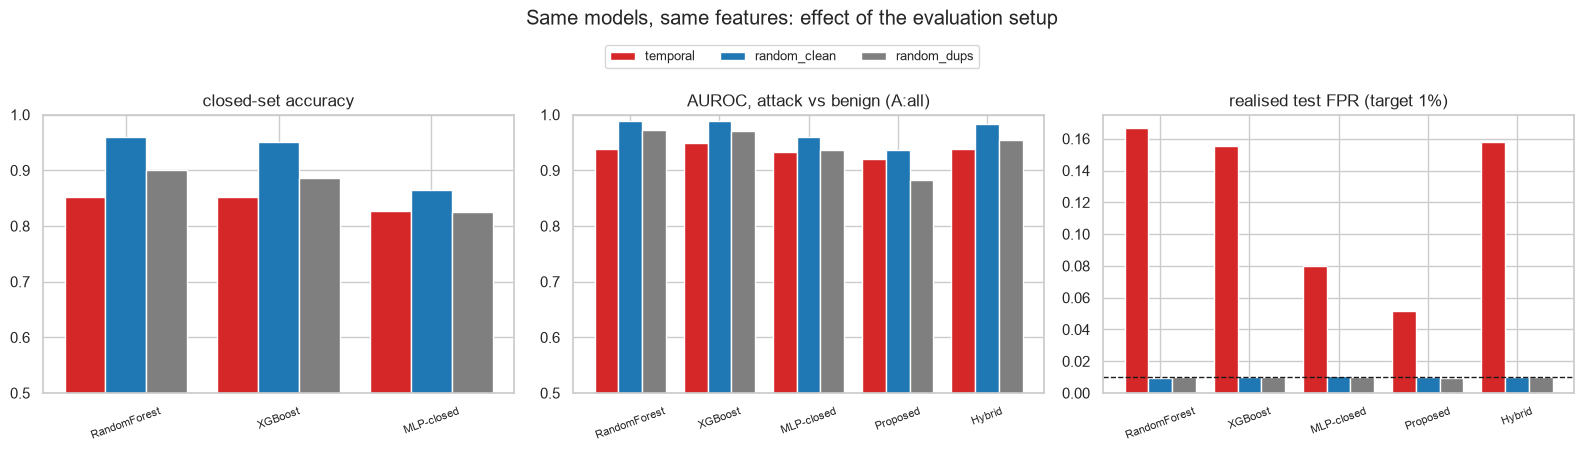
\includegraphics[width=0.78\textwidth]{figs/fig_split_effect.png}
\caption{Same models under different evaluation setups: closed-set accuracy (left), AUROC (middle) and realised FPR against the 1\% target (right).}\label{fig:split}
\end{figure*}

\textbf{Methodological comparison:} Against OHCE and HERO, a 7,092-parameter MLP on flow statistics replaces convolutional or graph encoders on packet bytes, and a calibrated maximum of two prototype distances replaces the Hamming-ball test, targeting cost (G2). Against EVADE and ET-SSL, the benign boundary is kept but the embedding is learned with attack labels and the threshold is set on validation data only. Against DC-GL and GCN-MHA, temporal splits replace random splits and single-flow CPU latency replaces time per epoch. Unlike all five, it is tested on held-out families and across datasets, and explains its alerts.

\textbf{Improvement analysis:} Against XGBoost, the strongest re-implemented baseline, AUROC is 0.028 lower ($-$2.9\%), but realised FPR is 10.0 points lower ($-$65\%), precision 0.181 higher (+34\%) and F1 0.028 higher (+4.2\%), with 3.1$\times$ lower latency and a 31$\times$ smaller model; the gain comes from the benign boundary, which reacts less to day-to-day drift than a tree posterior. Against the EVADE-style detector on the same data, AUROC improves by 0.489 because the learned embedding separates SSH and PortScan, which unsupervised PCA cannot. In reported cost, the detector is 1.9$\times$ faster than OHCE (CPU vs.\ GPU), 4.7$\times$ than EVADE, 40$\times$ than GCN-MHA (63$\times$ fewer parameters) and 39--66$\times$ than ET-SSL, on different hardware.

\textbf{Fairness:} The detector does \emph{not} exceed the reported accuracies of the base papers. Temporal splits (10.7 points), removal of duplicates and conflicts, and validation-only thresholds explain much of the gap; datasets, representations (no packets or graphs) and hardware also differ, and the hash-centre and graph models could not be re-implemented from flow CSVs. XGBoost remains significantly better at ranking known attacks.

%%==================================%%
\section{Ablation Study}\label{sec:ablation}
%%==================================%%

Table~\ref{tab:ablation} varies one component at a time (3 seeds). Removing TCP flags hurts most (0.920$\to$0.832), followed by timing, volume and length, so every group carries signal. A 5$\times$ smaller network (1,424 parameters) loses nothing and a 9$\times$ larger one gains only 0.006, so capacity is not the bottleneck (supporting G2). Using only the top-10/20/40 features lowers AUROC. Adding the port changes AUROC by 0.003, so the detector does not rely on it. On one trained network, the combined score (0.892) is close to its Proto-ratio component (0.897), above Benign-boundary (0.855) and far above MSP (0.519); its value lies in the lower realised FPR. All variants stay at 0.34--0.52 on unseen families, so no single component causes the G1 failure; the limit is the flow-statistics representation.

\begin{table}[t]
\caption{Ablation: AUROC of the proposed score (mean $\pm$ std, 3 seeds; Protocol B averaged over families).}\label{tab:ablation}
\footnotesize
\setlength{\tabcolsep}{2.5pt}
\begin{tabular}{@{}lcc@{}}
\toprule
Variant & A (known) & B (unseen) \\
\midrule
Full model (68 feat., 64-32-16) & 0.920$\pm$0.002 & 0.405$\pm$0.089 \\
Drop TCP flags & 0.832$\pm$0.003 & 0.341$\pm$0.186 \\
Drop timing & 0.899$\pm$0.002 & 0.423$\pm$0.203 \\
Drop volume & 0.903$\pm$0.016 & 0.503$\pm$0.090 \\
Drop length & 0.912$\pm$0.003 & 0.343$\pm$0.239 \\
Small net (16-8-4) & 0.920$\pm$0.005 & 0.355$\pm$0.183 \\
Large net (256-128-64) & \textbf{0.926}$\pm$0.004 & 0.408$\pm$0.222 \\
Top-10 features & 0.862$\pm$0.008 & 0.495$\pm$0.089 \\
Top-20 features & 0.885$\pm$0.022 & 0.460$\pm$0.185 \\
Top-40 features & 0.904$\pm$0.012 & 0.446$\pm$0.240 \\
Add destination port & 0.923$\pm$0.008 & \textbf{0.518}$\pm$0.104 \\
\botrule
\end{tabular}
\end{table}

%%==================================%%
\section{Discussion}\label{sec:discussion}
%%==================================%%

\textbf{Why it works, and where it fails:} The compact embedding separates known attacks from benign traffic, and the robustly calibrated benign boundary reacts less to benign drift than an ensemble posterior, giving a nearly 3$\times$ lower realised FPR than XGBoost at sub-millisecond cost. Unseen families fail because, in flow-statistics space, an unseen family on an encrypted port lies closer to benign traffic than to any known attack: unseen SSH looks more normal than benign, and missed infiltration resembles HTTPS. All baselines and ablations fail in the same way, suggesting that packet-sequence or TLS-handshake features are needed.

\textbf{Practical implications:} A threshold chosen on validation days can give 5--16$\times$ the intended FPR later, so thresholds should be recalibrated routinely; this needs only about 1,000 unlabeled benign flows and tolerates 5\% contamination. Explanations add little overhead.

\textbf{Gap achievement:} G1 is \emph{not achieved}; G2 is \emph{achieved} (0.38\ms, 0.03\,MB, AUROC 0.922); G3 is \emph{partly achieved} (3/4 criteria, SSH transfer fails); G5 is \emph{partly achieved} (5/6 criteria, few unseen alerts to explain).

\textbf{Limitations and threats to validity:} The secure-port filter only approximates encryption. Family and dataset are confounded (PortScan only in 2017, Infiltration only in 2018, SSH only on port 22). Only flow statistics were available; CIC-IDS-2017 lacks timestamps; PortScan has 69 test flows and benign capping alters class ratios; 15 paired runs limit test power; latency was measured on a laptop CPU rather than edge hardware; v2 and v3 were designed after seeing earlier results; and infiltration labels are noisy.

%%==================================%%
\section{Conclusion and Future Work}\label{sec:conclusion}
%%==================================%%

This paper proposed a lightweight open-set detector for encrypted-port flows and evaluated it against seven re-implemented baselines under temporal splits and validation-only thresholds. It scores a flow in 0.38\ms{} on one CPU thread, detects known attacks with AUROC 0.922 at a much lower realised FPR than tree ensembles, can be recalibrated on a new network from 1,000 unlabeled benign flows, and its alerts are explained faithfully at low cost. Neither it nor any baseline detects unseen families from flow statistics, and random splits inflate reported accuracy. Future work should add packet-level or TLS-handshake features, use datasets with more shared attack families and explicit encryption labels, address drift with new classes (G4) and measure latency on edge devices.

\backmatter

\bmhead{Acknowledgements}
The authors thank Ms.\ Laraib (Computer Networks, FAST-NUCES) for guidance throughout this project, and the Canadian Institute for Cybersecurity for the public datasets.

\section*{Declarations}
\textbf{Funding:} none. \textbf{Competing interests:} none. \textbf{Ethics:} not applicable (public, anonymised data). \textbf{Data availability:} CIC-IDS-2017 and CSE-CIC-IDS2018 are public \cite{kaggle2017,kaggle2018}; all preprocessing steps and counts are given in Section~\ref{sec:setup}. \textbf{Code availability:} the full implementation, including the notebook \texttt{24i-0053\_24i-0061\_Phase3\_CNET.ipynb} and this manuscript's \LaTeX{} source, is available at \url{https://github.com/Ru-1234/AI-Intrusion-Detection-Encrypted-Traffic}.
\textbf{Reproducibility:} seeds 0--4; ports, caps, split, threshold, architecture and optimiser settings are given in Sections~\ref{sec:method}--\ref{sec:setup}; Random Forest/XGBoost use 100 trees (RF depth 20), Isolation Forest 100 trees, recalibration 1,000 flows, EG 64 references and KernelSHAP 200 samples. \textbf{Author contributions:} both authors contributed equally to all parts of the work. \textbf{Use of AI tools:} Claude (Anthropic) was used to help structure and typeset this manuscript from the authors' Phase~1--3 reports; all experiments, code, results and interpretations are the authors' own, and the authors checked every number and take full responsibility for the content.

\bibliography{references}

\end{document}
